\subsection{Dll's erzeugen und einbinden (FA)}
\label{DLLs_HOWTO}
Nachfolgend eine kurze Erklärung, wie man 'Dynamic Link Libraries' (kurz dll's) in Qt mithilfe des QtCreators und Visual Studio erzeugt und diese dann wiederum in ein beliebiges Programm einbindet. Als weitere Anleitungen bieten sich \cite{Dll_1} und \cite{Dll_2} an, welche eine Beschreibung für den QtCreator bieten und Teile von \cite{Dll_3}, die einige Einstiegsinformationen für Visual Studio enthalten. Am besten eignet sich jedoch die Video-Tutorials unter \cite{Dll_4} und \cite{Dll_5}, welche detaillierte Erklärungen liefern..

\subsubsection{Qt-Creator}
Zunächst muss ein neues Projekt für die dll erstellt werden. Hier muss als Vorlage 'C++-Bibliothek' gewählt werden, welche die nötigen Eigenschaften einer dll innerhalb des Projektes automatisch setzt (siehe Abbildung \ref{fig:proj}). \newline
\begin{figure}[H]
	\centering
	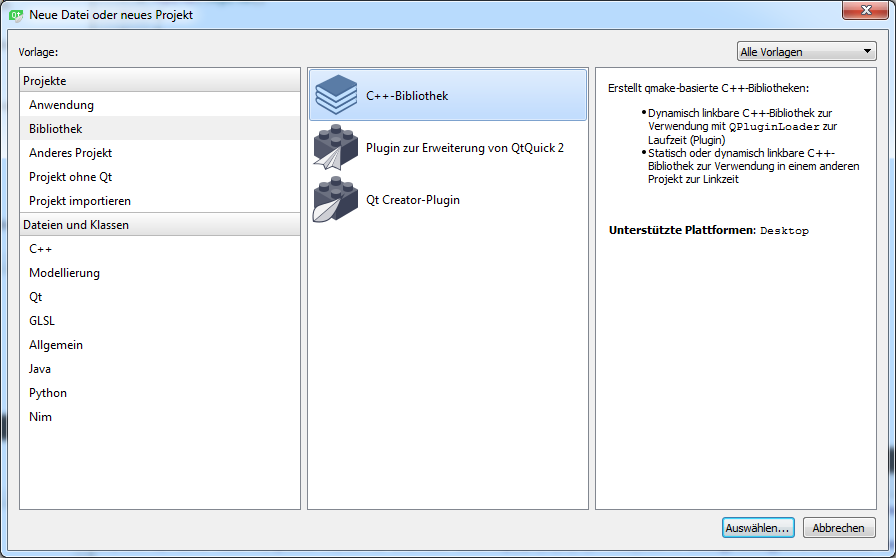
\includegraphics[width=0.90\textwidth]{figures/qtProjekt.png}
	\caption{Auswahl des Projekttyps}
	\label{fig:proj}
\end{figure}
Daraufhin ist es wichtig, die markierte Option 'dynamisch gebundene Bibliothek' auszuwählen (siehe Abbildung \ref{fig:bib}). Hier könnte man auch eine statische Bibliothek erzeugen, dies interessiert allerdings nicht.
\begin{figure}[H]
	\centering
	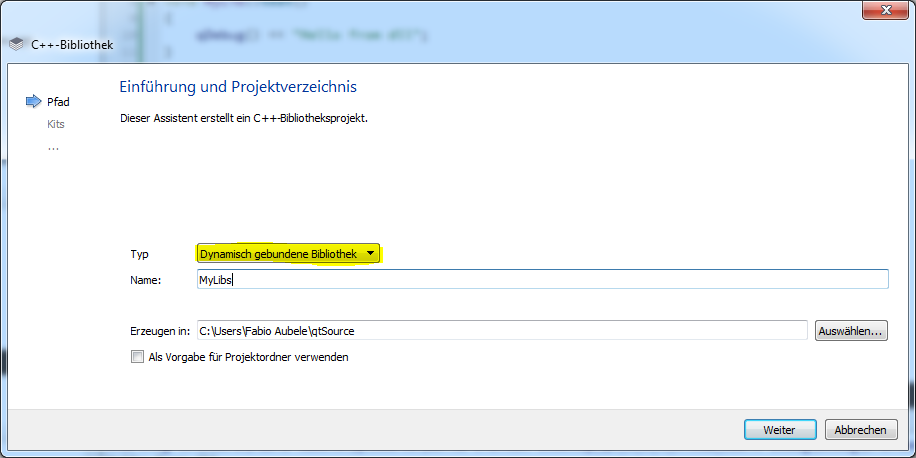
\includegraphics[width=0.90\textwidth]{figures/qtAuswahl.png}
	\caption{Auswahl des Bibliothekstyps}
	\label{fig:bib}
\end{figure}
Bei der Wahl des Compilers ist es wichtig KEINEN der Visual Studio Compiler (abgekürzt durch MSVC) auszuwählen, sondern MinGW (siehe Abbildung \ref{fig:comp}). Dies hat den Grund, dass Visual Studio eine etwas andere Form von DLLs erstellt, welche innerhalb des QtCreators beim Einbinden Fehler aufwerfen, da die DLL nicht lesbar ist.
\begin{figure}[H]
	\centering
	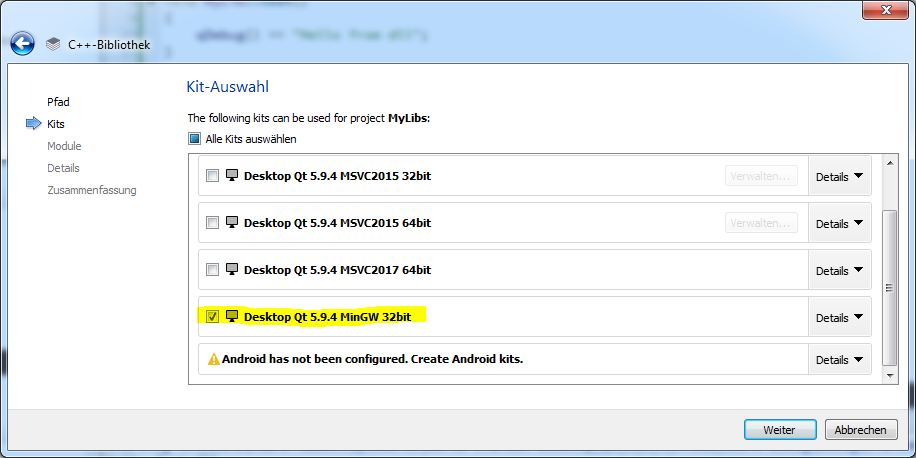
\includegraphics[width=0.90\textwidth]{figures/qtCompiler.png}
	\caption{Auswahl des Compilers}
	\label{fig:comp}
\end{figure}
Die restlichen Einstellung können beliebig abgeschlossen werden.\newline
Daraufhin kann das Projekt frei wählbar um weitere Dateien, Funktionen oder Klassen ergänzt werden. Wichtig ist, dass jede Header-Datei den globalen Header inkludiert (Im Beispiel: 'mylib\_global.h', siehe Abbildung \ref{fig:head}). Dahingegen muss jede Klasse in der Header-Datei das festgelegte Präfix am Anfang der Deklaration stehen haben (Im Beispiel: 'MYLIBSHARED\_EXPORT', siehe Abbildung \ref{fig:head}), dies gilt auch für Funktionen außerhalb von Klassen. \newline
Der globale Header wird automatisch bei der Erstellung des Projektes generiert. Dieser definiert den eben erwähnten Präfix, welcher sicherstellt, dass es sich um eine DLL handelt.
\begin{figure}[H]
	\centering
	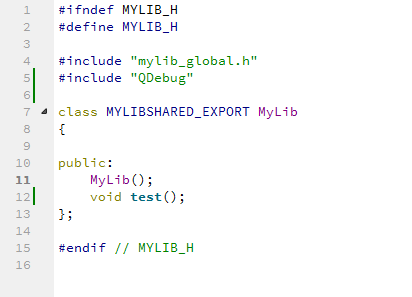
\includegraphics[width=0.40\textwidth]{figures/qtAufbau.png}
	\caption{Aufbau einer Header-Datei}
	\label{fig:head}
\end{figure}
Das Projekt, welches die DLL einbindet, kann ein zum Beispiel beliebiges GUI-Projekt sein, sollte aber auch nicht mit einem Visual Studio Compiler erstellt worden sein. In diesem müssen die Header-Dateien in das neue Projekt hinzugefügt werden. Dies sollte man in einem extra 'Include-Ordner' (zum Beispiel 'include' genannt) machen, damit die Übersicht über die Dateien leichter beibehalten werden kann. Ebenfalls muss die erzeugte DLL-Datei mit der dazugehörigen '*.a-Datei' in das neue Projekt hinzugefügt werden. Dafür sollte ebenfalls ein zusätzlicher Ordner erstellt werden (zum Beispiel 'lib' genannt). In diesen Ordner die '*.dll-Datei' hinzufügen. Daraufhin muss die Bibliothek der Applikation bekannt gemacht werden. Dies geschieht mithilfe des Dialogs unter Abbildung \ref{fig:Pro}.
\begin{figure}[H]
	\centering
	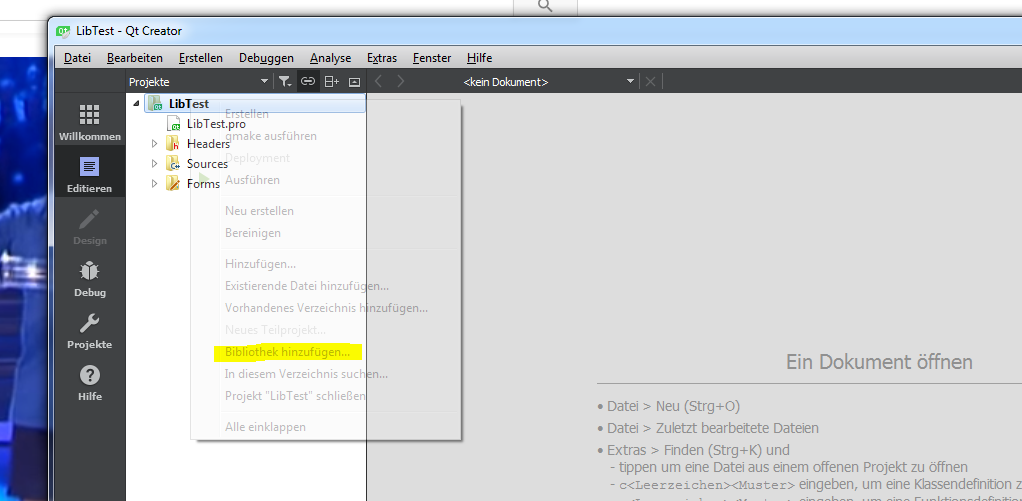
\includegraphics[width=0.60\textwidth]{figures/qtPro.png}
	\caption{Bibliothek hinzufügen}
	\label{fig:Pro}
\end{figure}
Hier wählt man 'externe Bibliothek', daraufhin öffnet man unter 'Bibliotheksdatei' die '*.a-Datei', welche man in den erstellten 'lib-Ordner' gezogen hat. In Abbildung \ref{fig:bibdatei} sieht man beispielhafte Einstellungen, welche bis auf die Pfade übernommen werden können. 
\begin{figure}[H]
	\centering
	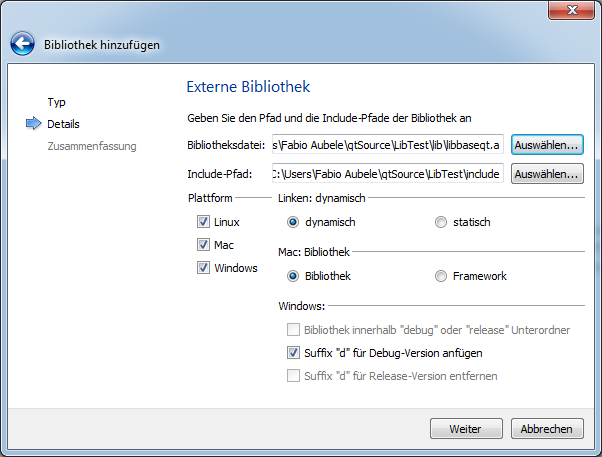
\includegraphics[width=0.40\textwidth]{figures/qtBibdatei.png}
	\caption{Einstellungen für die Bibliothek angeben}
	\label{fig:bibdatei}
\end{figure}
Dies bereitet das System auf die dll vor und legt Einträge in der 'pro-Datei' an. Debug und Release Versionen werden hier nicht berücksichtigt. \newline
Nun muss nur noch der gewünschte Header inkludiert und die Funktion oder Klasse aufgerufen werden (siehe Abbildung \ref{fig:Final}).
\begin{figure}[H]
	\centering
	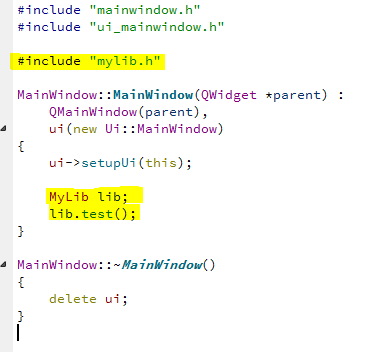
\includegraphics[width=0.30\textwidth]{figures/qtFinal.png}
	\caption{Aufruf der dll}
	\label{fig:Final}
\end{figure}

\subsubsection{Visual Studio}
Das Erzeugen einer dll läuft in den selben Schritten ab wie oben beschrieben. Einzig die Oberfläche der Dialoge ist etwas anders und die Voreinstellung des Projektes lautet 'Qt Class Library' und nicht 'C++-Bibliothek'. \newline
Auch das Editieren des dll-Projektes läuft exakt gleich ab und die vorgefertigten Dateien sind gleich aufgebaut. Jetzt zu den Unterschieden. Als Ausgabe bekommt man hier nicht nur eine '*.dll-Datei', sondern auch eine '*.lib-Datei'. Beide Dateien sind wichtig beim Einbinden der dll. \newline
\newline
Zum Einbinden kann wieder eine beliebige Gui-Applikation dienen. Anfänglich müssen im Verzeichnis der Applikation wieder zwei neue Ordner erstellt werden. Einmal ein 'include-Ordner', hier werden wieder die gewünschten Header-Dateien hinzugefügt und zusätzlich auch der global-Header, wie auch oben beschrieben. Des Weiteren wird auch ein 'lib-Ordner erstellt, hier wird jedoch die '*.lib-Datei' und nicht wie oben die '*.dll-Datei' hinzugefügt. In Abbildung \ref{fig:ordner} sieht man die Ordnerstruktur, markiert sind hier die neuen Ordner.
\begin{figure}[H]
 	\centering
 	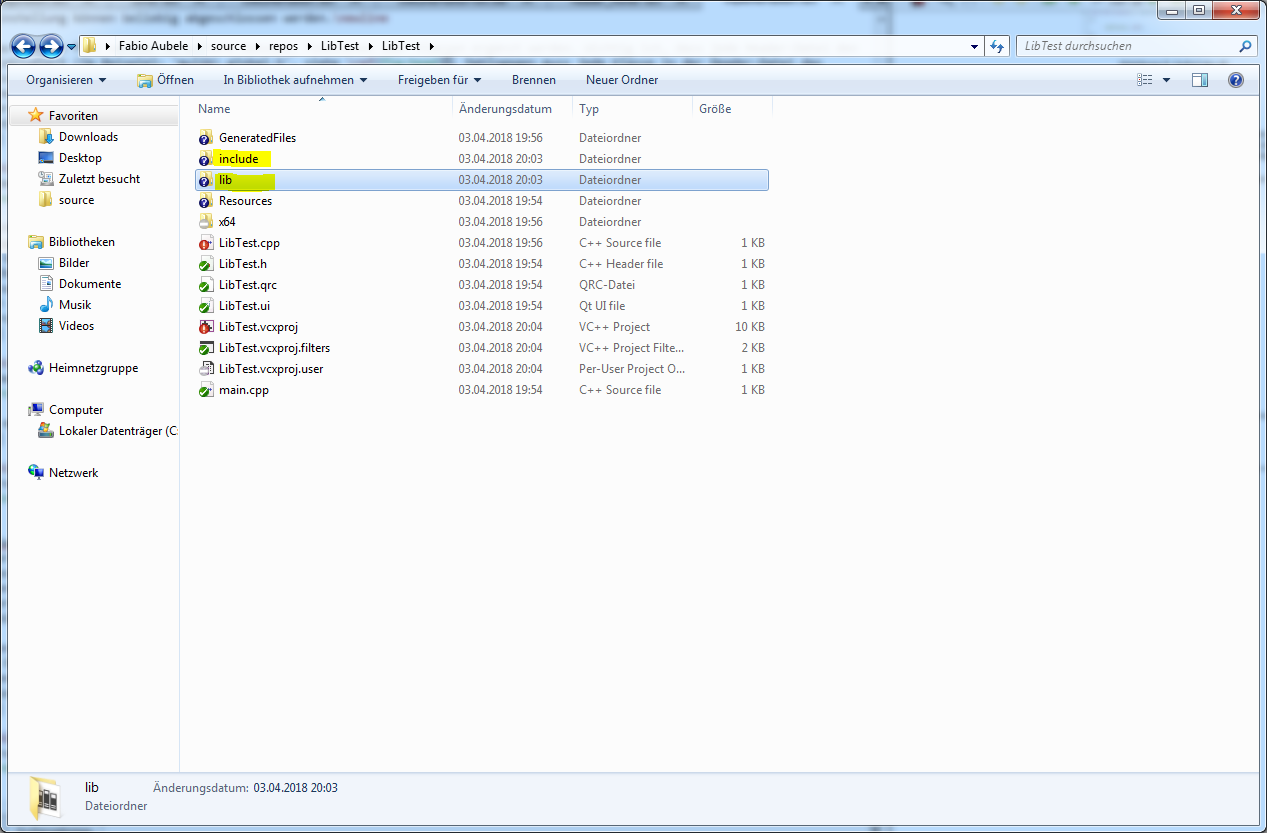
\includegraphics[width=0.80\textwidth]{figures/vsOrdner.png}
 	\caption{Ordnerstruktur}
 	\label{fig:ordner}
\end{figure}
Nun müssen einige Projekteinstellungen geändert werden, damit Visual Studio die neuen Verzeichnisse und Dateien erkennt und benutzt. Zunächst muss der Include-Ordner bekannt gemacht werden, dies ist unter Projekt -> Projekteigenschaften -> C/C++ -> Allgemein -> Zusätzliche Includeverzeichnisse zu tun. In Abbildung \ref{fig:inc} sieht man den hinzugefügten Eintrag:
\begin{figure}[H]
	\centering
	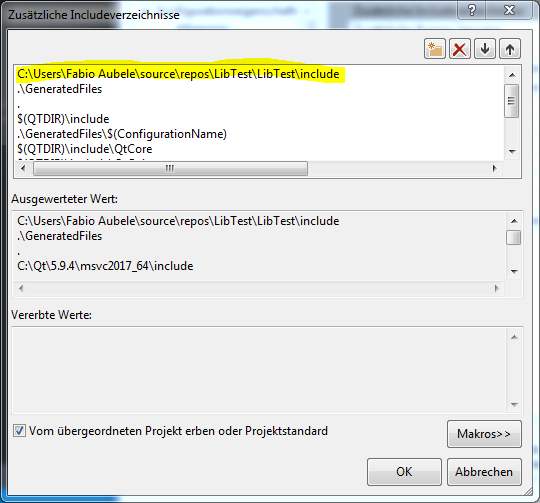
\includegraphics[width=0.40\textwidth]{figures/vsInclude.png}
	\caption{Eintrag des Includeverzeichnisses}
	\label{fig:inc}
\end{figure}
Daraufhin ist der 'lib-Ordner' preiszugeben. Dies geschieht unter Projekt -> Projekteigenschaften -> Linker -> Zusätzliche Bibliotheksverzeichnisse. In Abbildung \ref{fig:bibV} sieht man den Eintrag:
\begin{figure}[H]
	\centering
	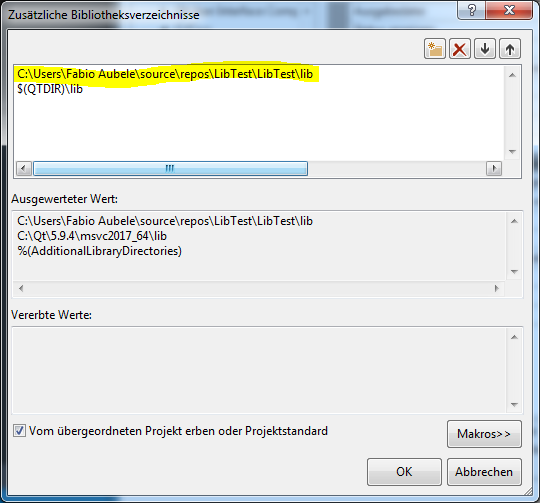
\includegraphics[width=0.40\textwidth]{figures/vsBib.png}
	\caption{Eintrag des Bibliotheksverzeichnisses}
	\label{fig:bibV}
\end{figure}
Schlussendlich muss Visual Studio noch der Name der Datei innerhalb des 'lib-Ordners' mitgeteilt werden. Dies ist möglich unter Projekt -> Projekteigenschaften -> Linker -> Eingabe. In Abbildung \ref{fig:bibV2} sieht man den Eintrag:
\begin{figure}[H]
	\centering
	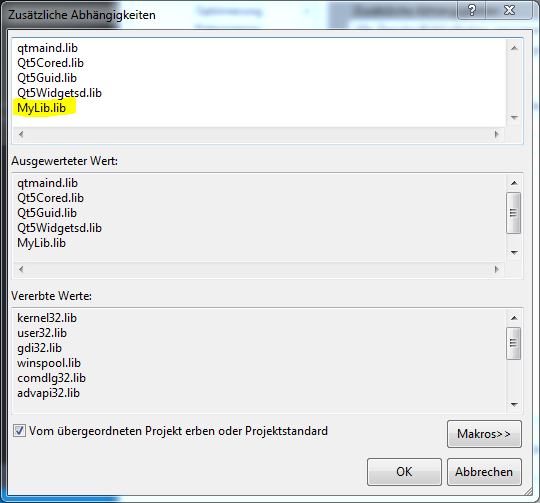
\includegraphics[width=0.40\textwidth]{figures/vsBib2.png}
	\caption{Eintrag der Bibliothek}
	\label{fig:bibV2}
\end{figure}
Zum Schluss muss in das Build-Verzeichnis, in welchem auch die '*.exe-Datei' liegt, die '*.dll-Datei' hinzufügt werden (meist unter x64 -> Debug oder x86 -> Debug). Nun kann man die gewünschte Header-Datei inkludieren und je nach Belieben Funktionen und Klassen aufrufen (siehe Abbildung \ref{fig:Final2}).
\begin{figure}[H]
	\centering
	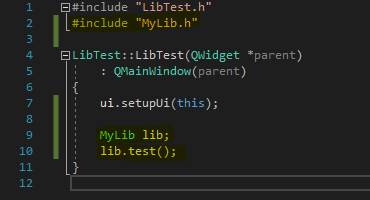
\includegraphics[width=0.40\textwidth]{figures/vsFinal.png}
	\caption{Aufruf der dll}
	\label{fig:Final2}
\end{figure}
\newpage